% -*- latex -*- This is a LaTeX document.
% $Id: pldi02.tex,v 1.12 2001-11-16 20:08:47 cananian Exp $
%%%%%%%%%%%%%%%%%%%%%%%%%%%%%%%%%%%%%%%%
\documentclass[preprint]{acmconf}
% don't forget to turn off 'preprint' before submission!
%\usepackage[section,plain]{algorithm}
%\usepackage{amsthm} % proof environment
%\usepackage{amstext} % the \text command for math mode (replaces \mbox)
\usepackage{varioref} % \vref command
\usepackage{graphicx} % for eps figures
\usepackage{color}
\usepackage{comdef}
\newcommand{\figscale}{1.0}

%setup varioref package
\renewcommand{\reftextbefore}{on the preceding page}\vrefwarning

\newcommand{\mycomment}[1]{}

\title{\bf Data Size Optimizations for Java Programs}

\author{C.~Scott~Ananian \\
	Laboratory for Computer Science\\
	Massachusetts Institute of Technology\\ 
	Cambridge, MA 02139 \\ 
	{\tt cananian@lcs.mit.edu} }

\begin{document}
% in preprint mode, tag pages with a revision identifier.
\pagestyle{myheadings}\markboth{$ $Revision: 1.12 $ $}{$ $Revision: 1.12 $ $}
\bibliographystyle{plain}

\maketitle

% abstract
\begin{abstract}

This paper presents a set of Java optimizations targetted at
memory-constrained embedded devices.  Using the FLEX compiler system,
we aggressively transform
programs using both source-level transformations and
specializations of the runtime environment to save as much
as {\bf XX}\% of the storage requested by the allocator.

Our techniques fall into three broad categories: header optimizations,
bitwidth analyses, and mostly-zero field elimination.  Header
optimizations reduce the size penalties associated with 
Java's virtual dispatch, hashcode, and locking features.  Bitwidth
analyses allow compile-time reduction of field sizes when the
full range of a datatype is unused.  Mostly-zero field elimination
attempts to factor out fields which are ``usually zero'' (as
determined by profiling) to obtain savings.  Combined, these
techniques allow the compiler to shoulder the burden of space accounting
and allow the use of general-purpose software on extremely
memory-constrained embedded devices.

\end{abstract}

% outline for paper.
% introduction
\section{Introduction}
The devices around us are getting dramatically smarter, but the
processing capabilities of your average toaster will always remain far
inferior to those of a desktop computer.  Nevertheless, the designers
of embedded devices would like to use the high-level software
languages and paradigms designed for the desktop environment when
programming their much smaller systems.  The past few years have
demonstrated a remarkable industry push to run software written in
languages such as Java on cellphones, PDAs, and similar platforms.
At the moment, much of this desire is for downloaded applets and
extension programs and upgrades; for firmware the slight
inefficiencies of the high-level languages, multiplied by the large
quantities of devices deployed, warrant lower-level approaches.

The aim of this paper is to present optimization and analysis
techniques to close this gap.  There is as much as a four-fold
% maybe more! reference here?
cost difference between ROM and RAM costs in embedded devices,
so we will concentrate on reducing the dynamic heap usage of
programs written in Java.  We will bypass the difficulties of
real-time control
for the moment, and assume that running-time of the optimized programs
is not important (so long as it is reasonable); we will trade-off
slight increases in execution time and ROM usage for dramatically
reduced RAM usage.

We will first present header optimizations which tweak the runtime's
representation of non-field information in Java objects in order to
reduce memory consumption.  We will then turn our attention to
compressing the values stored in object fields.  Using static
analysis, we will determine the minimal number of bits required to
represent a field's contents, and then present three alternate
field-packing techniques to take advantage of the unused bits
identified.  For systems with small memories, pointer compression is
also discussed.

Finally, we will attempt to identify ``mostly-constant'' information in
objects, specializing the object to reduce the space required for
the common case.  For fields which are not mutated, we statically
specializing the class to remove predictable values;
for mutable fields we utilize an
external hashtable to store values which are rarely unpredictable.

These optimizations were implemented using the FLEX compiler
infrastructure and Java runtime \cite{flexweb}.  FLEX is a
whole-program compiler which generates native code, but many of these
techniques are also applicable to open-world JVM environments.

We present the results of applying our optimizations to the SPEC
benchmark suite --- a set of general tasks, which, although they may bear
little relation to actual programs one would want on an embedded
device, span a gamut sufficient to adequately show the strengths and
weaknesses of our techniques.

% graph showing breakdown of allocated memory: header, pointers, fields.

\section{Header Optimizations}
% header optimizations
%  discussion of typical object layout.
%  claz compression.
%  hashcode/lock compression.
%   analyses for doing so; static/dynamic hash counts.

The Java language specification requires that several pieces of
information about an object be stored in addition to the data in its
fields.  Most obviously, information about the {\it class} or {\it
  type} of the object must be available in order to implement dynamic
dispatch and primitives such as {\tt instanceof}.  In addition, there
must be some way to associate a synchronization lock with each object,
and each object must have a {\it identity hash code} associated with
it to facilitate hashtable implementations of various kinds.%
\footnote{Arrays must, in addition, contain a specification of their
  length; we treat the length as a standard {\tt int} field of the
  object in this paper.  Although not discussed at length in this
  paper, the techniques of bitwidth analysis, etc, are equally valid
  when applied to this field.}
A typical implementation uses two words of header information in
addition to the fields contained by the object.  The first, often
designated {\tt claz}, is a pointer to a class descriptor structure for the
object's type.  Dynamic dispatch is usually implemented as an
indirection through a table contained in this descriptor.
The second word is usually overloaded to contain both hashtable and
lock information.  Although the declaration of the {\tt
  Object.hashCode() } and {\tt System.identityHashCode()} methods
return a 32-bit {\tt int}, implementations usually return some
more restricted range of values --- one implementation of IBM's JDK
\cite{bacon98}
returned as little as 8 bits of hashcode.  The remaining bits of the
second word are used to represent the lock and any other information
kept by the runtime.  In the FLEX compiler system used for this
research 30 bits of hashcode are kept, and the
remaining 2 bits in the word indicate whether the value is actually a
hashcode or
a pointer to an ``inflated'' object structure containing
a displaced hashcode, pthreads locks,
and other runtime information.

\subsection{{\tt claz} compression}
The first and most obvious means of reducing the size of the header
kept for each object is to replace the direct class descriptor
pointer with an index into a table.  For the closed-world systems
expected on embedded devices, the number of program classes is known
and may be compiled into the program.  For extensible systems, one may
instead define epochs of execution in which the number of classes
in the system is bounded; between epochs a full-system garbage
collection may be necessary to expand the size of the index in the
header, but epoch transistions should be rare.%
\footnote{Alternatively, a
variable length encoding could be used so that ``young'' class types
(hopefully the most common classes) may be given short indices without
limiting the index size as the class universe grows.  The runtime cost
of such a scheme is likely to be prohibitive, however.}

Table \ref{tab:claz-space} shows the number of classes required to
build each of
the spec benchmarks, as determined by a standard class hierarchy
analysis at compile-time.  Also enumerated are the heap savings to be
expected from reducing the size of the {\tt claz} information using
table-lookup, for both bit and byte packings of the {\tt claz} index
(these packing alternatives will be discussed further in
section \ref{sec:field-packing}).  The {\tt claz} field accounts for an
average of 12\% of the total bytes allocated by our benchmarks, and we
can reclaim roughly three-quarters of that.
\begin{table}
\begin{tabular}{lcr@{.}lr@{.}l}
&& \multicolumn{4}{c}{\bf \% alloc'ed space saved} \\
\bf Benchmark &\bf \# classes & \multicolumn{2}{c}{\bf std/byte} &
                             \multicolumn{2}{l}{\bf~~bit} \\ \hline
200\_check	& 253 &  3&8\% &  3&8\% \\
201\_compress	& 216 &  0&0\% &  0&0\% \\
202\_jess	& 379 &  6&0\% &  8&6\% \\
205\_raytrace	& 239 & 14&4\% & 14&4\% \\
209\_db 	& 213 & 12&6\% & 12&6\% \\
213\_javac	& 399 &  6&8\% &  9&8\% \\
222\_mpegaudio	& 213 &  3&7\% &  3&7\% \\
227\_mtrt	& 239 & 14&4\% & 14&4\% \\
228\_jack	& 265 &  7&3\% & 10&6\% \\
\end{tabular}
\caption{Number of classes statically referenced in SPEC benchmarks,
  and the savings (in \% of total allocated bytes) of {\tt claz} field
  compression to nearest byte and bit boundaries.}
\label{tab:claz-space}
\end{table}

\subsection{Hashcode/lock compression}
Many objects in a typical Java program are neither locked nor inserted
into hashtables; thus the second word of the header is unused.
If we can determine that synchronization on an object is unnecessary
or never performed, that the hashcode is likewise never accessed,
and that any other runtime features signalled in the second header
word are unused, we can eliminate it from the object.

Determining that the lock features are unnecessary is straight-forward.
We use our previously published escape analysis
\cite{salcianu01,vivien01,whaley99}
to determine on which objects synchronization must be performed; we
can discard the lock bits of all the rest.  Hashcode utilization
is a little more involved: it is not sufficient to identify the
objects in which the system {\tt Object.hashCode()} method is
overridden and not invoked, because there is also a {\tt
  System.identityHashCode()} method in the library which provides the
same value on any object.  Standard type analysis around the
call sites in question will not help, because generic collection
classes such as {\tt java.util.Hashtable} typically invoke
the {\tt hashCode} method on the generic {\tt Object} type contained
in the collection.  Either context-sensitivity or a type-cone analysis
is necessary to obtain the needed precision.

In this investigation, we used a dynamic enumeration of classes on
which {\tt Object.hashCode()} or {\tt System.identityHashCode()} is
actually invoked at run-time.  This allows us to determine the
upper-bound on hashcode-related savings.  It may initially be
surprising to learn that only the 213\_javac benchmark ever invokes a
system hashcode method (on objects of only 8 types); but on reflection
this should be obvious: hashCodes tightly tied to the objects identity
(as opposed to its field contents) are typically only useful when some
guarantee of object uniqueness can be guaranteed.  But the obvious way
to guarantee that only one object has a given field contents is to
write a factory method which looks up the proposed new object in a
{\it field}-keyed hashtable.  This chicken-and-egg problem usually
assures that a field-based override of the {\tt Object.hashCode()}
method is implemented.

Since only the SPEC benchmark {\tt 227\_mtrt} is multithreaded
(making it trivial to determine that object locking is unnecessary
for the other benchmarks)
and only {\tt 213\_javac} contains
any objects which require hashcodes, we find that we can completely
eliminate the second header word from all objects in 7 of our 9 benchmarks.
Table \ref{tab:hashlock-opt} presents the number of classes on which
hashcodes and locks are required for each of our benchmarks, and the
space savings due to eliminating the second header field when it is
unused.
\begin{table}
\begin{tabular}{lccr@{.}l}
&\multicolumn{2}{c}{\bf\# classes requiring:}&\multicolumn{2}{c}{\bf\% alloc'ed}\\
\bf Benchmark &\bf hashcodes&\bf locks&\multicolumn{2}{c}{\bf space saved}\\\hline
200\_check	&   0 &   ~0   &  5&1\% \\
201\_compress	&   0 &   ~0   &  0&1\% \\
202\_jess	&   0 &   ~0   & 12&0\% \\
205\_raytrace	&   0 &   ~0   & 19&2\% \\
209\_db 	&   0 &   ~0   & 16&8\% \\
213\_javac	&   8 &   ~0   & 13&6\% \\
222\_mpegaudio	&   0 &   ~0   &  5&0\% \\
227\_mtrt	&   0 &   17   & 19&0\% \\
228\_jack	&   0 &   ~0   & 14&7\% \\
\end{tabular}
\caption{Number of classes in SPEC benchmarks which dynamically use
  the hashcode and lock features of the second header word,
  and the savings (in \% of total allocated bytes) of unused header/lock
  elimination.}
\label{tab:hashlock-opt}
\end{table}

\section{Field compression}
% field compression.
%  description of bitwidth analysis.
%   treatment of loops.
%   constant/unread fields.
%   scc.  crib from thesis.
%   interprocedural.  no appreciable gain from context sensitivity.
%   no pointer analysis to discriminate object classes (yea, type-safety)
%  implementation: bit/byte/java-type packing.
After the header has been reduced in size as much as possible, we turn
our attention to the values contained in the object fields.
The key idea here is to
do a {\it bitwidth analysis} \cite{ananian99:tech,stephenson00}
to determine an upper bound on
the number of bits required to represent all values stored in
the field.  We can then shrink the size of the field consistent with
this bound, subject to
limitations on field and object alignment.  
A straight-forward implementation with strongly-aligned objects and
field widths restricted to those of standard Java types will achieve
modest space reductions with very little implementation effort; these
gains are achievable even when running in a JVM environment.
The largest savings require eliminating as many alignment restrictions
as possible, which will typically require substantial changes to the
runtime system.

\subsection{Bitwidth analysis}
Our bitwidth analysis is an inter-procedural extension of that
described in \cite{ananian99:tech}.  It is based on Wegman and
Zadeck's Sparse Conditional Constant (SCC) propagation algorithm
\cite{wegman91:scc}, with extensions to a bitwidth lattice.
Since almost all types in Java are signed (with the exception of the
16-bit {\tt char}), we must handle both negative and positive numbers.
We first extend the basic three level value lattice of Wegman and
Zadeck to allow the classification of negative, positive, or zero
values, as illustrated in figure~\ref{fig:scclat6}.
A join on two negative numbers yields the entry \code{(M--)}, a
join on a negative and a positive number yields \code{(M-P)}, and so on.
\begin{figure}
\centering\renewcommand{\figscale}{0.6}\input{Figures/THlat6}
\caption[An integer lattice for signed integers.]
{An integer lattice for signed integers. A classification into
negative (M), positive (P), or zero (Z) is grafted onto the standard
flat integer constant domain.  The \code{(M-P)} entry is duplicated to
aid clarity.}
\label{fig:scclat6}
\end{figure}

Now substitute integers $M$ and $P$ into the tuples, to represent the
widths of the absolute value of the negative and positive portion of
the number.  Merging the constants $2$ and $4$ would result in the lattice
value \code{(--3)}, for example, and merging $-4$ with $4$ would result in
\code{(3-3)}.  Some combination rules for arithmetic operations are
shown in figure~\ref{fig:bitrules}.
\begin{figure}
\begin{eqnarray*}
-\tuple{M,P} &=& \tuple{P,M}\\
\tuple{M_l,P_l} + \tuple{M_r,P_r} &=& \tuple{1+\max(M_l,M_r),1+\max(P_l,P_r)}\\
%\tuple{M_l,P_l} \times \tuple{M_r,P_r} &=& \langle\max(M_l+P_r,P_l+M_r),\\
%                                       &&  \max(M_l+M_r,P_l+P_r)\rangle\\
\tuple{M_l,P_l} \times \tuple{M_r,P_r} &=&
\tuple{\begin{array}{l}\max(M_l+P_r,P_l+M_r),\\
                       \max(M_l+M_r,P_l+P_r)\end{array}}\\
\tuple{0,P_l} \wedge \tuple{0,P_r} &=& \tuple{0,\min(P_l,P_r)}\\
\tuple{M_l,P_l}\wedge \tuple{M_r,P_r} &=& \tuple{\max(M_l,M_r),\max(P_l,P_r)}
\end{eqnarray*}%
\caption{Some combination rules for bit-width analysis.  The \code{Z}
  element indicating whether zero is a possible value has been omitted
  for clarity.}\label{fig:bitrules}
\end{figure}

Dataflow on this bitwidth lattice is performed on the entire Java
program interprocedurally.  The analysis is what Heintze and Tardieu
\cite{heintze01}
would call {\it field-based}; that is, given a field $f$ defined in
class $X$, and an instance of $X$ named $x$, we consider an assignment
to $x.f$ to be an assignment to the field $X.f$ and ignore the base
object $x$.\footnote{An obvious extension is to use pointer
analysis to discriminate between fields allocated at different sites
in the program.}  The result of the analysis is a bitwidth
specification for each variable and field in the program.  As the
analysis is based on SCC, we also identify constant variables and
fields; reads of constant fields are replaced with their constant
value and the field is eliminated.  Fields which we do not discover
any reads of during our analysis are also removed as unused.
Table~\ref{tab:const-unused} shows the number of unused and constant
fields discovered by our analysis, and the dynamic space savings
realized by removing them.  With the exception of 202\_jess and
228\_jack, the objects containing most unused or constant fields are
very rarely instantiated.
\begin{table}
\begin{tabular}{lcccr@{.}l}
&\bf total&&&\multicolumn{2}{c}{\bf\% alloc'ed}\\
\bf Benchmark &\bf fields &\bf unread &\bf constant &
\multicolumn{2}{c}{\bf space saved} \\\hline
200\_check	& 279 &   79   &   35   &  2&6\% \\
201\_compress	& 298 &   75   &   31   &  2&5\% \\
202\_jess	& 485 &   91   &   43   &  9&9\% \\
205\_raytrace	& 341 &   75   &   30   &  0&0\% \\
209\_db 	& 286 &   75   &   35   &  0&0\% \\
213\_javac	& 531 &   85   &   34   &  0&6\% \\
222\_mpegaudio	& 286 &   75   &   35   &  1&4\% \\
227\_mtrt	& 341 &   75   &   30   &  0&0\% \\
228\_jack	& 378 &   77   &   31   & 10&2\% \\
\end{tabular}
\caption{Number of unused and constant fields in SPEC benchmarks,
  and the savings realized (in \% of total dynamic allocated bytes) by
  removing them.}
\label{tab:const-unused}
\end{table}

\subsection{Field packing}
\label{sec:field-packing}

\begin{figure*}
\centering
\begin{tabular}{|l|}
\hline
Standard packing word-aligns the object and aligns each field to the
width of its type (4-byte data is 4-byte aligned):\\
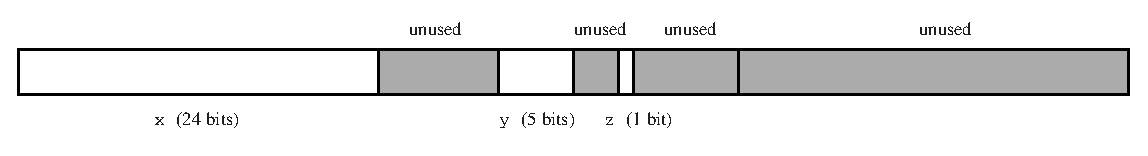
\includegraphics[scale=0.7]{Figures/standardAlignment.eps}\\
``Byte'' alignment byte-aligns the object and all fields:
\hfill\raisebox{-1ex}[0pt][0pt]{\parbox[t]{3in}{
\begin{samplecode}
class A \{\\
\>int x;  /* actual width 24 bits */\\
\>byte y; /* actual width 5 bits */\\
\>boolean z; /* actual width 1 bit */\\
\}\\
\end{samplecode}
}}\\
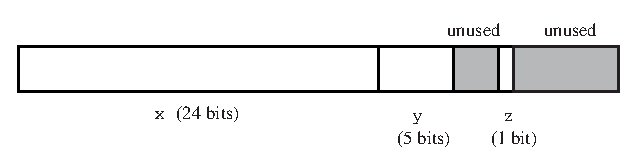
\includegraphics[scale=0.7]{Figures/byteAlignment.eps}\\
``Bit'' alignment requires not alignment of objects or fields:\\
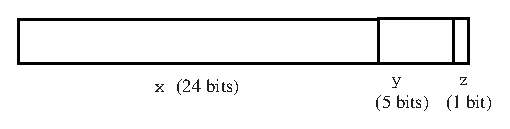
\includegraphics[scale=0.7]{Figures/bitAlignment.eps}\\
\hline
\end{tabular}
\caption{An example of different field packing scenarios.  The object
  header has been omitted for clarity.}
\label{fig:packing}
\end{figure*}

If the program is going to run on a standard java virtual machine, or
for some other reason modifications to the runtime environment are not
possible, then optimization based on the bitwidth analysis can only
shrink each field to the size of a standard Java type: 1,
8, 16, 32, or 64 bits.%
\footnote{The Java language specification allows, but does not mandate,
  a true 1-bit representation for booleans.  Many JVMs pad boolean
  elements out to an 8-bit type.}
The entire object will be padded so that
consecutive objects are properly aligned, most often to a word or
double-word boundary.  This scenario is labelled ``std'' in our results.

If we can modify the runtime, however, much better use may be made of
the information gleaned from bitwidth analysis.  For example, we can
allow field widths of any integral number of bytes, and pad/align
objects to byte boundaries, instead of words.  This entails some
cycle overhead on machines which disallow unaligned accesses, but is
fairly straight-forward to implement.  When this is done,
a 33-bit-wide field will
end up occupying a byte-aligned 40 bits (5 bytes), instead of the 64
bits (8 bytes) that the ``std'' scenario would require.  We will refer
to this implementation as ``byte''.

However, we can improve even this result.  If maximum space reduction
is desired, we can {\it bit}-align fields within a word.  Further, we
can bit-align objects as well by shifting our pointers left by 3 and
using the new lower-order bits to encode a bit-within-the-byte offset.
This requires much more time overhead to decode pointers and fields.
This scenario is called ``bit''.
%
Figure~\ref{fig:packing} illustrates the three different packing
scenarios for an illustrative class.

Note that all but the most aggressive form of the {\it bit} scenario
requires some amount of object padding.  In a space-conscious
compiler, careful attention must be paid to field layout to reduce
the ``holes'' caused by alignment restrictions, when present.  Our
field layout algorithm keeps a list of alignment-induced ``free
space'' within the object, and always attempts to fill a hole before
increasing the object size.  This means that small fields of a
subclass may end up being slotted {\it between} aligned fields of its
superclass.  This violates the ``traditional'' superclass-first
ordering of object fields, but does not pose any special problems.

Table {\bf XXX} shows the allocation reductions due to our bitwidth
analysis under each of the above scenarios.  We can see that {\bf blah
  blah blah.  ``bit'' does best, of course.}

Recall also table \ref{tab:claz-space}, which shows that aggressive
field packing can benefit header compression as well.

\subsection{Pointer compression}\label{sec:ptrcmp}
% sub-topic: pointer compression.
%  present numbers: how your memory stacks up.
The bitwidth analysis only produces results for fields of integer type.
However, fields with reference type constitute {\bf XX}\% of
the field bytes allocated.  These fields can be compressed, too:
typically an embedded system will not require a full 32-bit address
space,\footnote{Not to mention a 64-bit address space!} due to
limitations on the amount of memory and I/O address space actually attached
to the device.  If we are byte- or bit-packing our fields already,
it is straight-forward to implement sub-word widths for fields of
reference type.  Figure~{\bf XX} shows the expected space savings
across our benchmarks as one shrinks the pointer size.  A
space-optimizing java compiler ought to be able to specialize the code
emitted for the address space size of the target device to take
advantage of these potential savings.

\section{Mostly-zero field analysis}
% mostly-zero field analysis.
%  as extension: mostly-'N'
%  techniques:
%   dynamic specialization
%    analyses required.
%   ``external fields''
%    profiling/analyses required.
%    implementation of external hashtable.

Mostly-zero field analysis attempts to take advantage of commonly
recurring field values to reduce the space consumption of an object.
For example, the {\tt java.lang.String} class in the Java standard
library (see figure~\ref{fig:string-fields}) uses {\tt offset} and
{\tt count} fields to index into a character array, allowing the
implementation of the substring operation in constant time (without
copying data from the {\tt String}'s underlying character array into a
new array).  However, all of {\tt String}'s public constructors
initialize the {\tt offset} field to zero.  The single private
constructor which does otherwise is used only in the implementation of
the {\tt substring()} method.  So we can reasonably expect the vast
majority of the {\tt String} objects created in a typical program to
have a zero {\tt offset} field.  We use dynamic selection of
statically specialized classes to eliminate the field when its value
is the ``common'' one (zero in this case).  Where this transformation
is inappropriate, we
can use an external storage technique to only store ``uncommon''
values of the field.
\begin{figure}
\begin{samplecode}
public final class String \{\\
\>private final char value[];\\
\>private final int offset;\\
\>private final int count;\\
\>\ldots\\
\>public char charAt(int i) \{\\
\>\>return value[offset+i];\\
\>\}\\
\>public String substring(int start) \{\\
\>\>int noff = offset + start;\\
\>\>int ncnt = count - start;\\
\>\>return new String(value, noff, ncnt);\\
\>\}\\
\}\\
\end{samplecode}
\caption{Portions of the {\tt java.lang.String} class.}
\label{fig:string-fields}
\end{figure}

\subsection{Static specialization of near-final fields}
For fields which are effectively {\tt final}---i.e. not modified after
assignment in the constructor---we can split the class containing the
field into a ``small'' version without the field and a ``large''
subclass containing the field.  Without loss of generality, assume
that all field accesses have been transformed into calls to setter and
getter methods.  The ``small'' class will have a getter method
which will simply return the constant zero.  The ``large''
subclass will actually consult the field (which is only present in the
``large'' version of the class) and return or set its value (in the
getter and setter, respectively).  Figure~\ref{fig:big-small} illustrates this
conversion for a illustrative fragment of a {\tt java.lang.String}
implementation.
\begin{figure}
\begin{samplecode}
public final class SmallString \{\\
\>private final char value[];\\
\>private final int count;\\
\>int getOffset() \{ return 0; \}\\
\>\ldots\\
\>public char charAt(int i) \{\\
\>\>return value[getOffset()+i];\\
\>\}\\
\}\\
public final class String\\
\>\>extends SmallString \{\\
\>private final int offset;\\
\>int getOffset() \{ return offset; \}\\
\}\\
\end{samplecode}
\caption{Static specialization of {\tt java.lang.String}.}
\label{fig:big-small}
\end{figure}

This transformation is only correct for fields which are immutable
after their initialization.  However, since in our implementation
subclasses of the
original class will inherit from the ``large'' version of the class,
subclasses are allowed to mutate these fields.  We will say that
a class is {\it subclass-final} if the only writes to the field
are contained in constructors of its type and methods of its
subclasses.  Writes to the field within constructors must occur only on
the {\it this} object.

Some class constructors will always yield objects with zero-valued fields.
We can replace these instantiation expressions
with instantiations of the new ``small'' class.  Many constructors,
however, initialize (at least some) fields with simple functions of their
parameters.  To handle these cases, we also allow {\it dynamic
  selection} of the instantiated class.  In particular, if we can
prove that a field is zero iff a certain constructor parameter is
zero, then we can insert a test at the instantiation site to select
the small class if the parameter is zero, or else to use the large class.
An example of this approach on code which might constitute an
implementation of {\tt String.substring()} is shown in
figure~\ref{fig:dyn-select}.  Notice that rewriting the return type of the
method is necessary to ensure consistency with the new split
classes; in general, mentions of the split class in field/method signatures,
array creation expressions, and {\tt instanceof} tests must be
similarly widened for proper type-checking.

{\bf MORE INFO HERE? Maybe numbers on how many call sites use constant
  versus parameter-dependent tests?  Details on the analysis used?}

\begin{figure}
\begin{samplecode}
public SmallString substring(int start) \{\\
\>int noff = offset + start;\\
\>int ncnt = count - start;\\
\>if (noff==0)\\
\>\>return new SmallString(value, noff, ncnt);\\
\>else\\
\>\>return new String(value, noff, ncnt);\\
\}\\
\end{samplecode}
\caption{Dynamic selection among specialized classes in a method
  from {\tt java.lang.String}.}
\label{fig:dyn-select}
\end{figure}

\subsection{Creating external fields}
It is often the case that promising mostly-zero fields do not satisfy
the requirements for the static specialization transformation
described above.  The compiler may not be able to prove that mutation
of the field is impossible, or the value of the field may not be
easily predictable at the instantiation site.
{\bf For example, in jess\ldots } % XXX FIX ME.

In these cases, we can represent only the fields which have non-zero
values in an external map.\footnote{Note that this is roughly parallel
  to hashtable-based externalization of the putative ``lock'' field
  required in every object by the Java language specification; Bacon
  et al. give a brief description of this common
  practice in \cite{bacon98}.}
% indeed there is a deep symmetry between object fields and maps.
The savings are tempered by the requirement of storing a key along
with the value in the table, and for constructing a ``sufficiently
large'' hashtable so that searches will be efficient.  Typically this
approach is only worthwhile if more than 75\% of the allocated fields
are zero-valued.  The transformation is straight-forward: accesses to
the field in question are replaced by calls to getter/setter methods,
and then the field is eliminated and the getter/setters rewritten
to query the external map.

\subsubsection{External hashtable implementation}
Close attention to the implementation of this external map is
necessary to realize the gains possible in theory.  In order to
maximize space savings, it is necessary to utilize as little space
per field stored in the table as possible.  The overhead of
dynamically allocated buckets and the required {\it next} pointers
makes separate chaining impractical as an implementation technique
for all but fields with very few non-zero entries.  Open-addressing
implementations are preferable: in addition to the value being stored,
all that is necessary is a key value and the empty space required to
limit the load-factor.  A load factor of two-thirds and one-word keys
and values yield an average space consumption of three words per
field.  This implementation breaks even when the mostly-zero fields
identified are zero over 66\% of the time.

Key-size reduction is an important component of the implementation:
a na{\"\i}ve approach
would combine a one-word reference to the virtual-container object and a
one-word field identifier for a two-word key.  The large key will
shift the break-even point up so that only fields which are 82\% zero
will profit.  Instead, we can offset the
object reference (up to the limit of its size) by small integers
to discriminate the externalized fields of the object, which yields
a single-word key.  This technique is
subject to object-size-dependent limits on the number
of class fields which may be externalized.  The pointer compression
techniques of section \ref{sec:ptrcmp} may also be applied to the
keys.

\subsection{Identifying mostly-zero fields}

{\bf write me}

\subsection{Mostly-$N$ analysis}
Although this section has concentrated on zero-valued fields for
clarity, we need not limit ourselves to these.  Our implementation of
these ideas actually collects profiling data on ``mostly-$N$'' values
with $N$ an integer in the range $[-5,5]$.

{\bf XXX} Note that if we are considering a non-zero N, then
  we must also prove that a write to the field occurs on every
  non-exceptional path through the constructor, to prevent the default
  'zero' value from leaking out.

{\bf MORE HERE.}

\section{Results}
% results/discussion.
%  present sum totals.
%  compress doesn't do so hot: show why.

% discuss: why are there unused/constant fields in programs?

\section{Related work}
% BW: usually register width, MMX (local variables).  Cite hardware.

\section{Conclusion}
% conclusion/future work.
%  better pointer analysis/separate out classes of objects.
%   (strings as motivating example: compress to byte[])
%  pointer encoding: more common pointers at lower addresses?
%  other stuff?


\bibliography{harpoon}

%\appendix
%\input{pldi02-appendix}
\end{document}
